\documentclass[sigchi-a, authorversion]{acmart}
\usepackage{booktabs} % For formal tables
\usepackage{ccicons}  % For Creative Commons citation icons
\usepackage{todonotes}

% Copyright
\copyrightyear{2019}
\acmYear{2019}
\setcopyright{rightsretained}
\acmConference[CHI'19 EA]{CHI Conference on Human Factors in Computing Systems Extended Abstracts}{May 4--9, 2019}{Glasgow, Scotland Uk}
\acmBooktitle{CHI Conference on Human Factors in Computing Systems Extended Abstracts (CHI'19 Extended Abstracts), May 4--9, 2019, Glasgow, Scotland Uk}\acmDOI{10.1145/3290607.3299038}
\acmISBN{978-1-4503-5971-9/19/05}

%\acmBadgeL[http://ctuning.org/ae/ppopp2016.html]{ae-logo}
%\acmBadgeR[http://ctuning.org/ae/ppopp2016.html]{ae-logo}

\begin{document}
\title{From the Lab to the OB Truck: Object-Based Broadcasting at the FA Cup in Wembley Stadium}

\author{Thomas R\"{o}ggla$^1$, Jie Li$^1$, Stefan Fjellsten$^4$, Jack Jansen$^1$,  Ian Kegel$^3$, Luke Pilgrim$^3$, Martin Trimby$^3$, Doug Williams$^3$, Pablo Cesar$^{1,2}$}
\affiliation{%
  \institution{\vspace{9pt}Centrum Wiskunde \& Informatica$^1$ \quad Amsterdam, The Netherlands}
  \institution{Delft University of Technology$^2$ \quad Delft, The Netherlands}
  \institution{BT Applied Research$^3$ \quad Ipswich, United Kingdom}
  \institution{ChyronHego AB$^4$ \quad Stockholm, Sweden}}

\affiliation{\vspace{9pt}\{t.roggla, jie.li, jack.jansen\}@cwi.nl, stefan.fjellsten@chyronhego.com, \{ian.c.kegel, luke.2.pilgrim, martin.trimby, doug.williams\}@bt.com, p.s.cesar@cwi.nl}

% The default list of authors is too long for headers.
\renewcommand{\shortauthors}{T. R\"{o}ggla et al.}


%
% The code below should be generated by the tool at
% http://dl.acm.org/ccs.cfm
% Please copy and paste the code instead of the example below.
%
\begin{CCSXML}
    <ccs2012>
        <concept>
            <concept_id>10003120.10003121.10003122.10011750</concept_id>
            <concept_desc>Human-centered computing~Field studies</concept_desc>
            <concept_significance>500</concept_significance>
        </concept>
        <concept>
            <concept_id>10003120.10003121.10003124.10010865</concept_id>
            <concept_desc>Human-centered computing~Graphical user interfaces</concept_desc>
            <concept_significance>100</concept_significance>
        </concept>
        <concept>
            <concept_id>10003120.10003121.10011748</concept_id>
            <concept_desc>Human-centered computing~Empirical studies in HCI</concept_desc>
            <concept_significance>100</concept_significance>
        </concept>
    </ccs2012>
\end{CCSXML}

\ccsdesc[500]{Human-centered computing~Field studies}
\ccsdesc[100]{Human-centered computing~Graphical user interfaces}
\ccsdesc[100]{Human-centered computing~Empirical studies in HCI}

\begin{abstract}
  While traditional live-broadcasting is typically comprised of a handful of
  well-defined workflows, these become insufficient when targeting multiple screens
  and interactive companion devices on the viewer side. In this case study, we describe the
  development of an end-to-end system enabling immersive and interactive experiences
  using an object-based broadcasting approach. We detail the deployment of this
  system during the live broadcast of the FA Cup Final at Wembley Stadium in
  London in May 2018. We also describe the trials and interviews we ran in the run-up
  to this event, the infrastructure we used, the final software developed for controlling and rendering
  on-screen graphics and the system for generating and configuring the live
  broadcast-objects. In this process, we learned about the workflows inside an OB
  truck during live productions through an ethnographic study and the challenges
  involved in running an object-based broadcast over the Internet, which we discuss
  alongside other gained insights.
\end{abstract}

\begin{marginfigure}
\vspace{3.6cm}
    \hspace*{-2cm}
    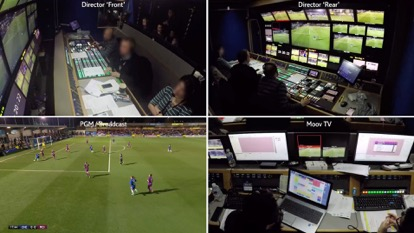
\includegraphics[width=9cm]{Figures/overview.jpg}
    \caption{Ethnographic study at the OB truck of Wembley Stadium (top) and Kingsmeadow Stadium (bottom), Uk}
    \label{fig:overview}
\end{marginfigure}

\keywords{Field study; user interface design; networking; object-based broadcasting; second screens; immersive experiences}

\maketitle

\section{Introduction}
 Live sport events are one of the mainstays of the television industry, since they bring
 the viewers close to the experience and enables them to enjoy the excitement of the
 event at home. The liveness is essential and cannot be reaplced by time-shifted on-demand viewing
 such as on Netflix~\cite{matrix2014netflix}.
 However, due to the unpredictable nature of a live sport event, this
 is challenging for the production team, also because the event does not take
 place in a studio. Live outside broadcasts are a world of well-defined
 workflows which deal with time-critical tasks. The roles inside an outside broadcast
 (OB) truck at a live sport event are divided by task, to capture
 the event while minimizing delays and mistakes (Figure~\ref{fig:overview}). Therefore, it is
 important that any software designed to supplement the workflow in an OB truck
 should be easy to operate, facilitate the collaboration within the production team
 and guarantee timely delivery of the live broadcast.

\begin{marginfigure}
\hspace*{-2cm}
    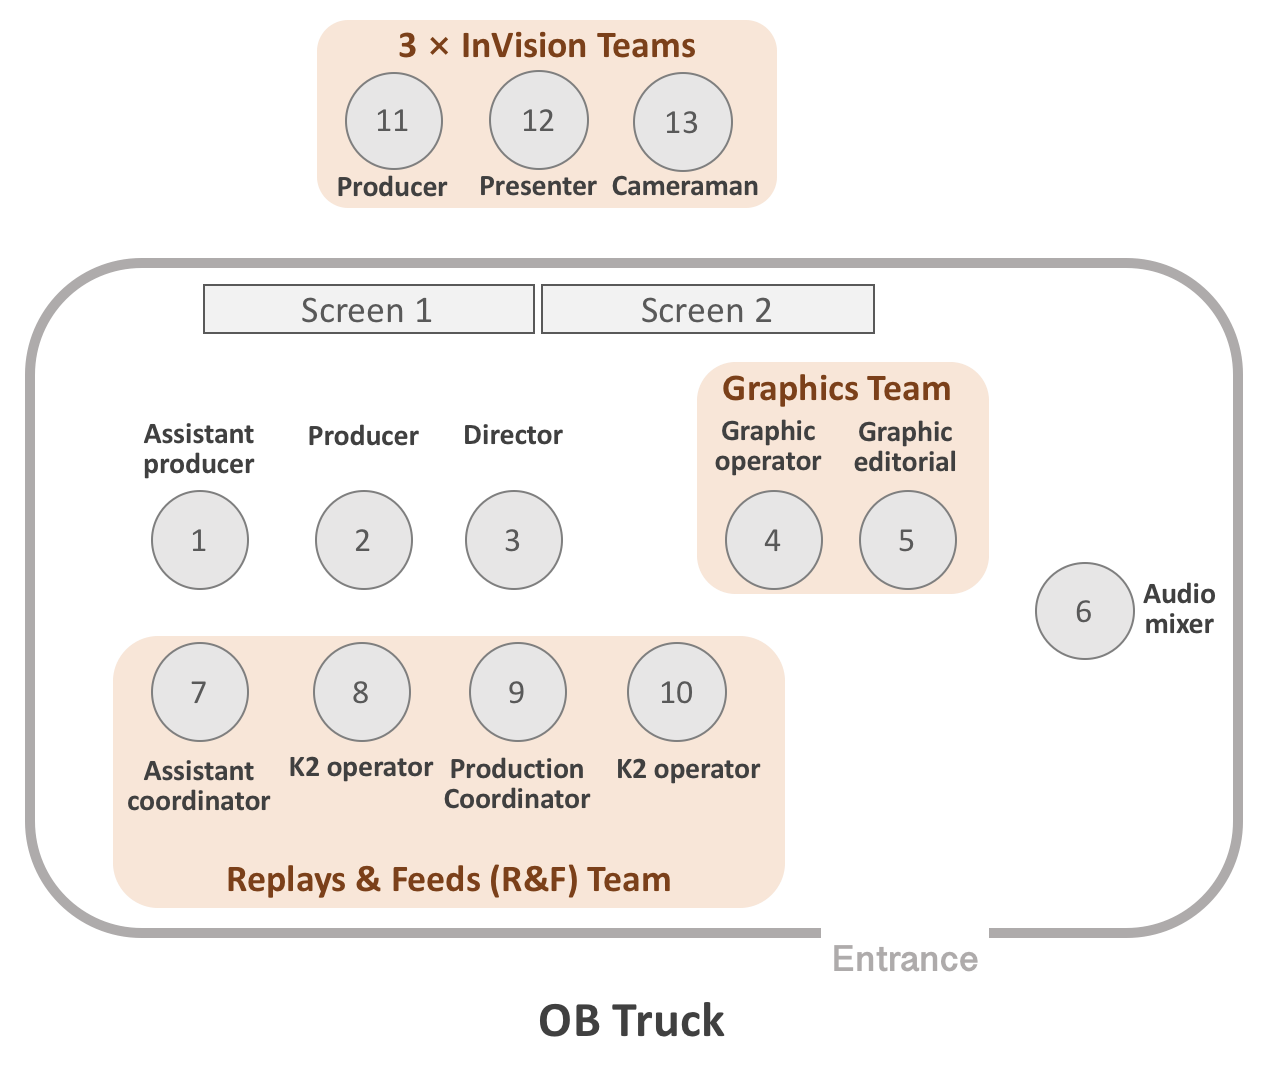
\includegraphics[width=10cm]{Figures/OBtruck.png}
    \caption{Layout of a typical OB truck used at a live sporting event}
    \label{fig:truck}
\end{marginfigure}

This case study presents the development and successful deployment of an
end-to-end platform for interactive, immersive broadcasts at
a live sports event. In particular, we detail the requirement gathering phase,
the aspects of the system used during the broadcast, including \emph{a graphics compositing
application}, a so-called \emph{Live Triggering} tool for inserting broadcast objects
into live streams, the camera setup, real-time encoding of video feeds and content
distribution over the Internet.
We show the path from a rough first prototype to a complete multi-user platform
with hardware integration. Finally, we also present a series of trials and
experiments that were completed along the way, culminating in the final
deployment of the system at the FA Cup final at Wembley stadium in London in
May 2018. There, the platform was used to support a test-broadcast of the
football match, delivering the experience to a number of viewers at
their homes.

At a big sports event such as this, an Outside Broadcasting (OB) truck is the most
common unit for live broadcasting. With its mobility, OB trucks can access any
location and work as a drive-in temporary production control center during live
transmission, providing complete video and audio facilities (Figure~\ref{fig:truck}).
An OB truck typically has a wall of monitors shared by all of the staff in the truck.
A video production switcher controlled by the director, an audio mixer, a team in
charge of recording and playback decks and a team responsible for live graphics.
It enables the production team to bring the TV audience an authentic
visual representation of an event as it is happening~\cite{owens2015}.
OB trucks vary in size depending on the scale of coverage and the nature of the
event. For a sport event, the coverage includes dozens of stationary cameras, a
couple of handheld cameras, cameras on motorcycles to capture the main athletes
and helicopters with cameras to shoot \emph{long-shots} of the
scene~\cite{owens2015, Li:2018_TVX}. Today, the production team in an OB truck
orchestrate smoothly to deliver the same linear live program to all kinds of TV
screens. The team typically follows a pre-scripted \emph{running order document} that
defines in detail where graphics, visual sources and sound come from and when
they should be put \emph{on-air}~\cite{Li:2018_TVX}.

As users at home often have multiple devices at their disposal (e.g.\ smartphones
and tablets) and these continue to be integrated
into standard television, a challenge production teams are facing is to tailor
the content of the TV program so that the content takes advantage of these
additional devices and screens. Content on companion screens is
customizable to provide the audience access to additional information next to the TV
screen, thus enabling interactive and immersive TV viewing
experiences~\cite{bentley2017, dowell2015}. However, given the current workload
of live broadcasting inside OB trucks, it is difficult to deliver additional
versions of the program to companion screens. New technologies are required for
this purpose~\cite{Li:2018_TVX, armstrong2014}. One such technology is
\emph{object-based broadcasting} (OBB). It allows the content of a TV program to
adapt to the requirements of different viewers on multiple screens, without
requiring the production team to separately produce different versions
of the program. The \emph{object}, here, refers to different media assets or content
objects that are used to make a TV program~\cite{armstrong2014}. The OBB approach
involves breaking down a program into separate objects, typically
media content such as graphics, audio, video, subtitles or effects and augmenting
it using metadata to describe how these objects can be
assembled on multiple screens. It enables the creation of a flexible, personalized,
and responsive program without increasing the production
workload~\cite{kegel2017, armstrong2014}. A rough layout of the production process
using our OBB system can be seen in Figure~\ref{fig:process}.

\begin{marginfigure}
    % \vspace{1pt}
    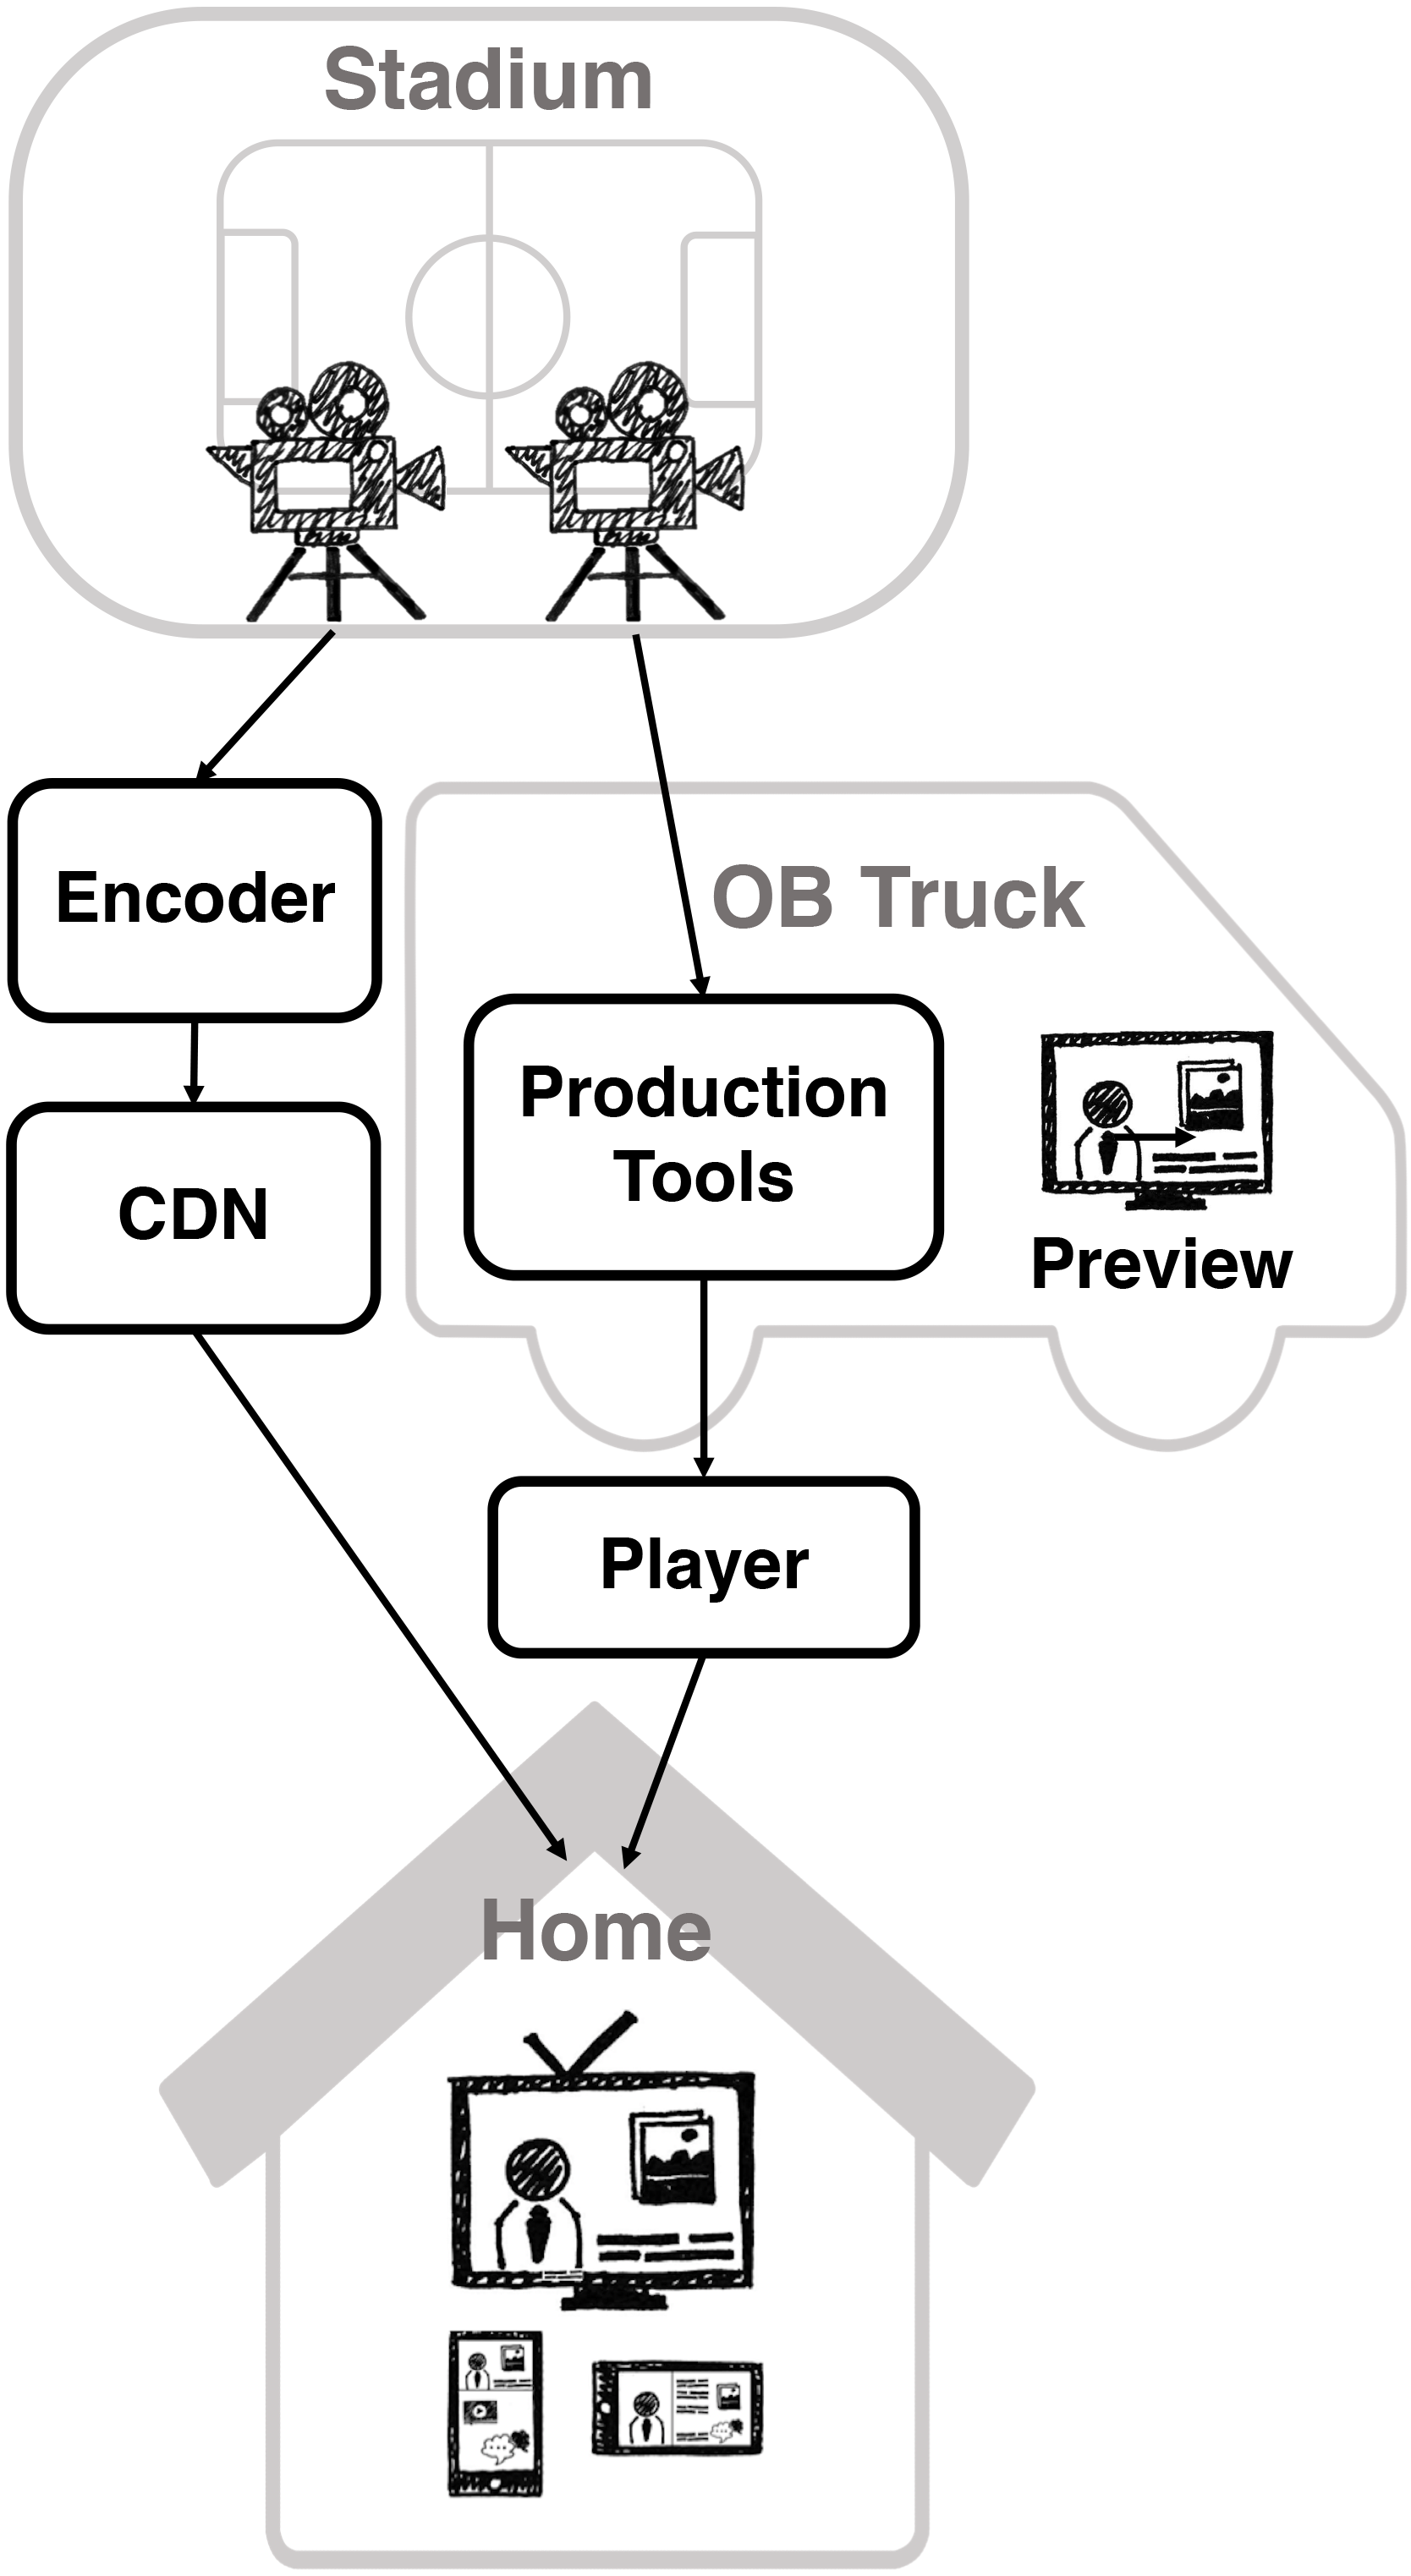
\includegraphics[width=7cm]{Figures/process.png}
    \caption{Production process for a live broadcast with our production platform. Content is recorded and edited on-premises and relayed to end-users via the Internet}
    \label{fig:process}
\end{marginfigure}

\section{Preparation}
Previously, we reported successful groundwork for the design and development
of a novel object-based broadcasting platform~\cite{kegel2017, Li:2018_CHI, Li:2018_TVX}.
Our next objective was its deployment during a live event like the FA Cup Final
2018 in Wembley. To better understand the challenges of delivering such a trial at
a live broadcast of a football match, the authors negotiated (via BT Sport) to be allowed
to observe the current processes inside an OB truck during a live event. In
particular, the following events were observed:

\begin{itemize}
  \item FA Community Shield match at Wembley Stadium on Sunday $6^{th}$ August 2017,
        where access was granted only to one match truck. This event provided us
        with an overview of the director's role in creating the broadcast mix of
        video, graphics and commentary narrative for the match;
  \item Women's Super League match at Kingsmeadow Stadium on Thursday $1^{st}$
        February 2018, where access was granted to observe and record inside the OB
        truck. A number of GoPro cameras were used to capture the pre-broadcast
        preparation and live broadcast activity within the main gallery of the
        truck. These videos were composited into a synchronized quad view video
        along with the broadcast output.
\end{itemize}

The capacity afforded by Wembley Stadium in terms of connectivity,
as well as physical gantry and production space, made it the preferred option as
an event venue. In addition to the more ethnographic observations detailed above,
the research team, working closely with the Chief Engineer and production team
at BT Sport, was allowed to run live tests during two matches at Wembley on $22^{nd}$
April 2018 (FA Cup Semi-Final) and on 12$^{th}$ May 2018 (National League Play-Off Final).

Such observations and tests resulted in a number of requirements, anticipating
operational and technological risks. Such requirements included, for example,
the creation of a number of documents such as the call sheet and the team sheet
(for pre-populating the graphics with the correct player names one hour before
the beginning of the match). The requirements also covered technological
aspects, such as the pre-production of the assets, the development of the
infrastructure to be deployed at the venue and in the cloud and the access to
various data channels such as clean video data feeds. Finally, there were
other operational guidelines for, for example, granting access to the researchers
or colocating our mini OB truck in the OB Compound with the other broadcasters.
The following subsections will detail the different preparation steps before the
official match day.

\subsection{Graphics}

\begin{marginfigure}
    % \vspace{2cm}
    \hspace*{-2cm}
    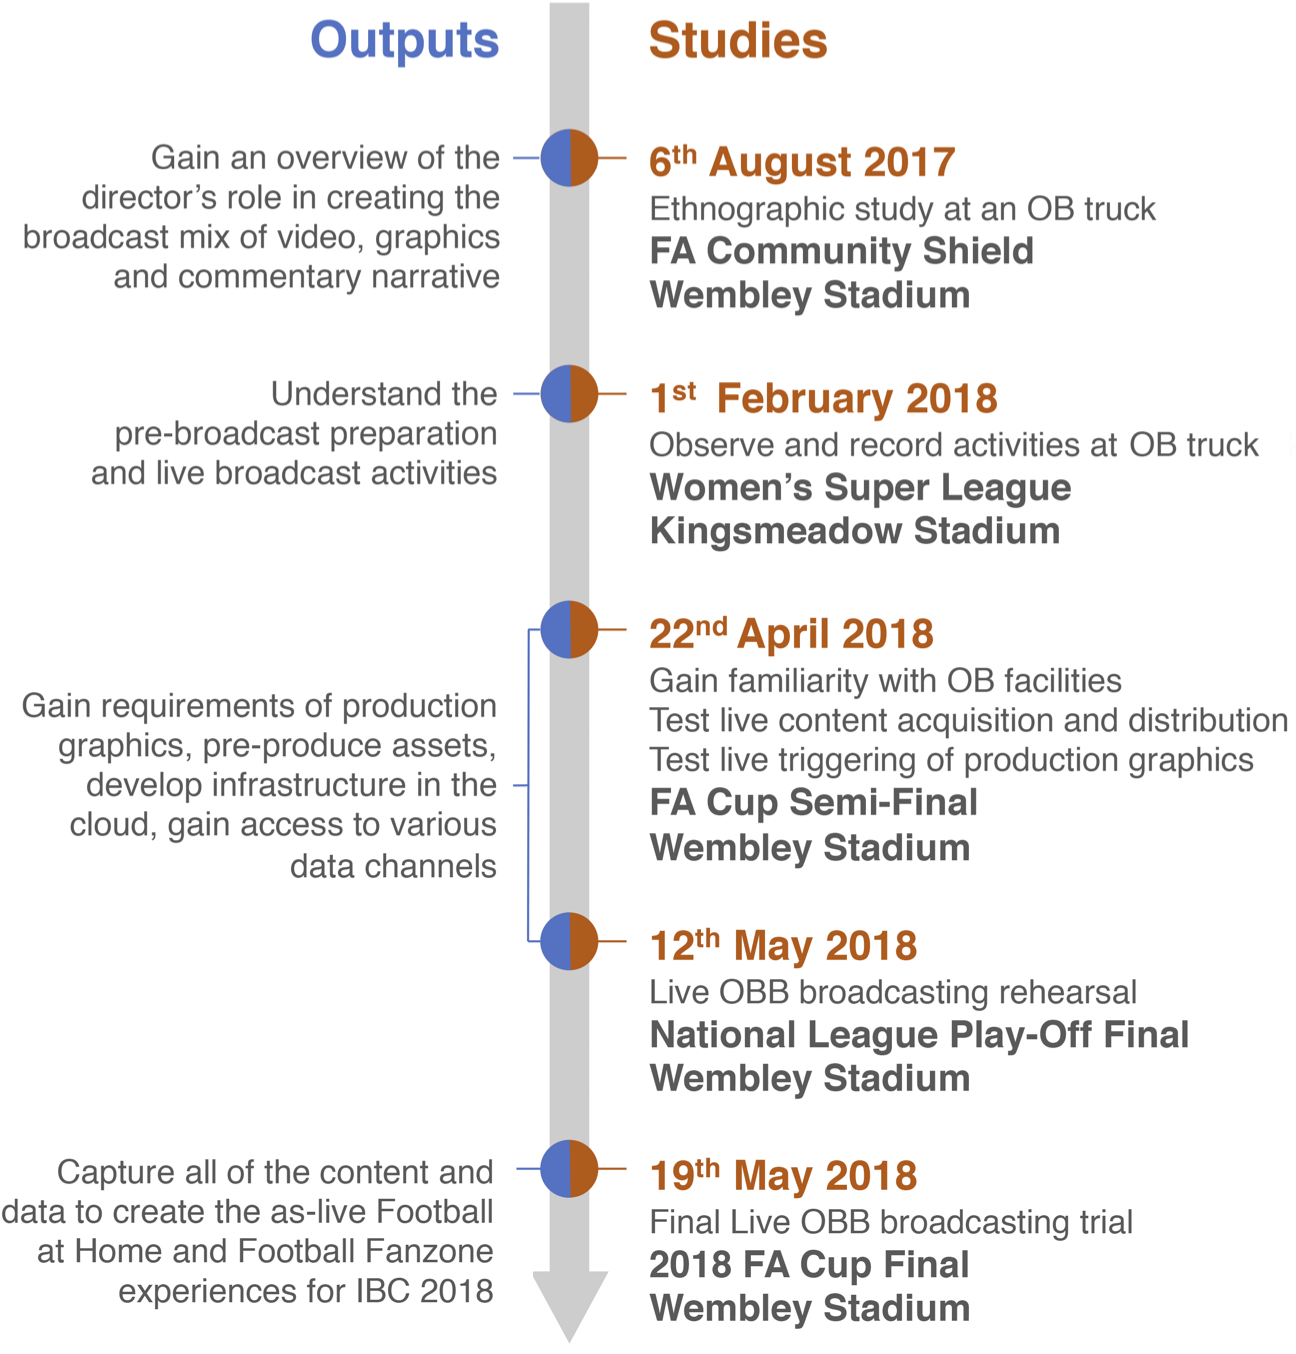
\includegraphics[width=10cm]{Figures/timeline.png}
    \caption{Timeline of the deployment of our end-to-end platform}
    \label{fig:timeline}
\end{marginfigure}

Object-based broadcasting provides user-level personalization and it thus
requires all broadcast graphics (non-video visualizations overlaid on top of
the video) to be composited on the client device. This is a major shift from
traditional broadcasts, where all graphics are overlaid and burnt into the
transmission signal at the OB truck. This requires new and more flexible ways
to author graphics. Experience from previous trials, where we took on a quite
developer-centric approach to coding such graphics in HTML and JavaScript,
showed that the process was cumbersome and time-consuming. The design of these
graphic elements and animations are valuable assets for a broadcaster and are
thoroughly defined and specified down to pixel perfection. For the FA Cup Final
we wanted to try out a more designer-friendly approach by utilizing an existing
broadcast WYSIWYG graphics authoring tool. The tool we choose was
\emph{ChyronHego Prime} (Figure 4). Using the ChyronHego Prime scene
description file format, the researchers created a specialized renderer for
object-based broadcasting which can execute Prime-authored graphics on the
client devices in real time. At the FA Cup Final, \emph{ChyronHego Prime} was also used for
creating the traditional broadcast graphics (4K HDR), so we were able to re-use
assets created for the broadcast graphics in our object-based broadcasting
workflow as well.

\subsection{Production Tool}

Previous work of the team resulted in a novel model and workflow for
production tools for object-based broadcasting~\cite{Li:2018_TVX,jansen2018}.
The tools were originally intended to cover MotoGP races, but we had the intuition that
they could be adapted for other sports as well. We thus arranged a number
of conversations with professionals working on TV sports broadcasts, asking them to
detail their experiences and workflows. We also carefully studied the recordings
from the OB truck at the FA Women's Super League game. Drawing upon these
observations, we concluded that our existing platform was a good starting point,
but required some modifications. First, all
controls needed to be easy to manipulate and target. Second, the person
preparing content for, e.g.\ replay clips is not the same as the
person who decides when and if the content is actually broadcast. The
former task is shared by several people, whereas the latter is usually performed
by either the director or a vision mixer. Finally, we learned that trucks
are equipped with special-purpose devices, providing direct access to
specific functions.

\begin{marginfigure}
    \vspace{-8cm}
    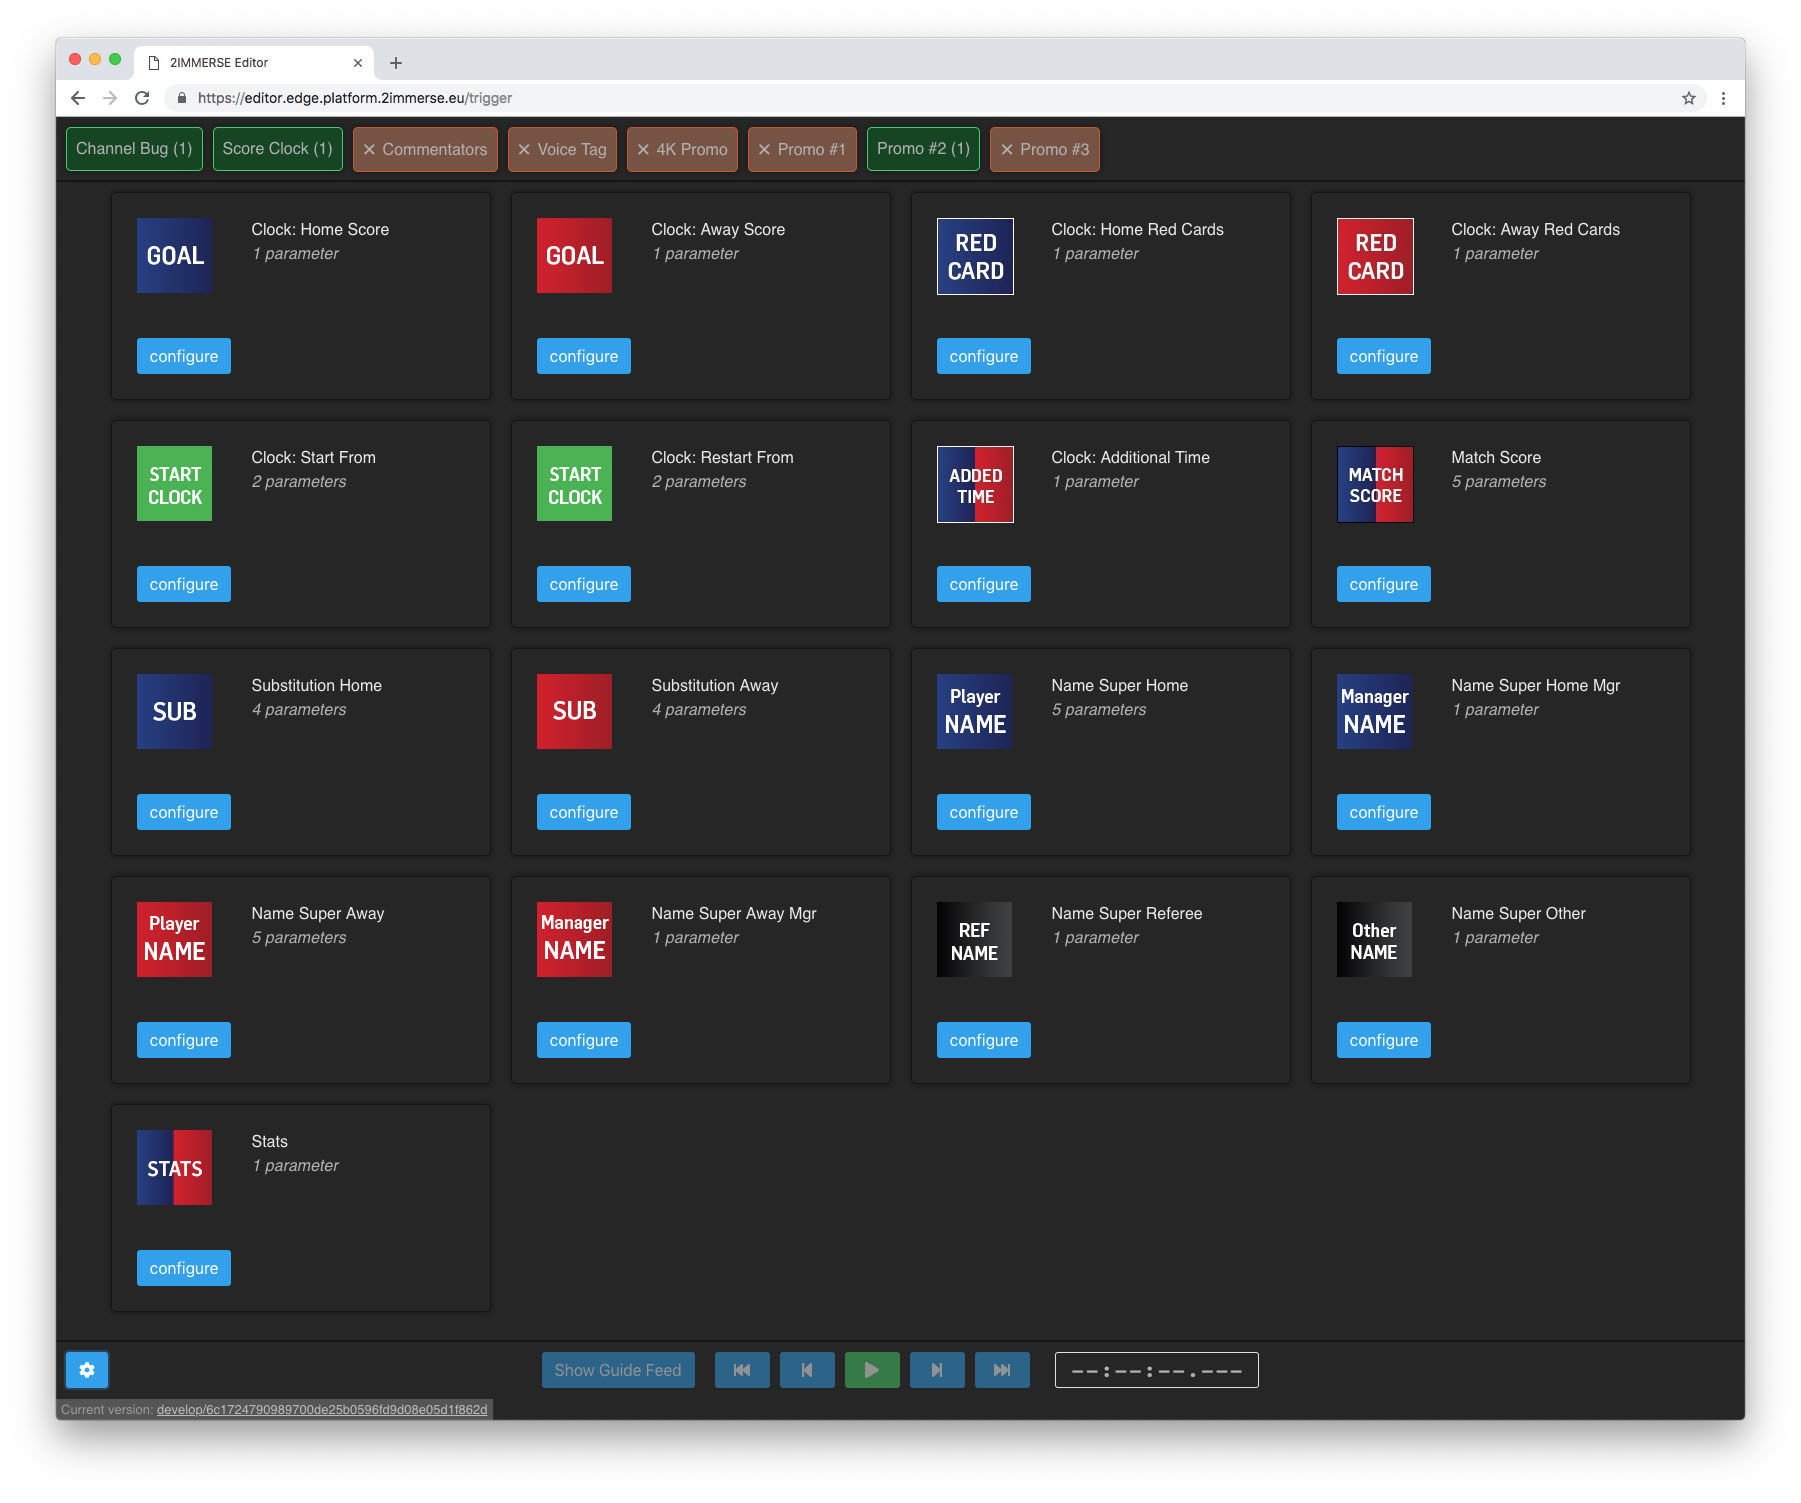
\includegraphics[width=\marginparwidth-10pt]{Figures/triggertool.jpg}
    \caption{Triggering tool in operation inside a web browser}
    \label{fig:triggertool}
\end{marginfigure}

\begin{marginfigure}
    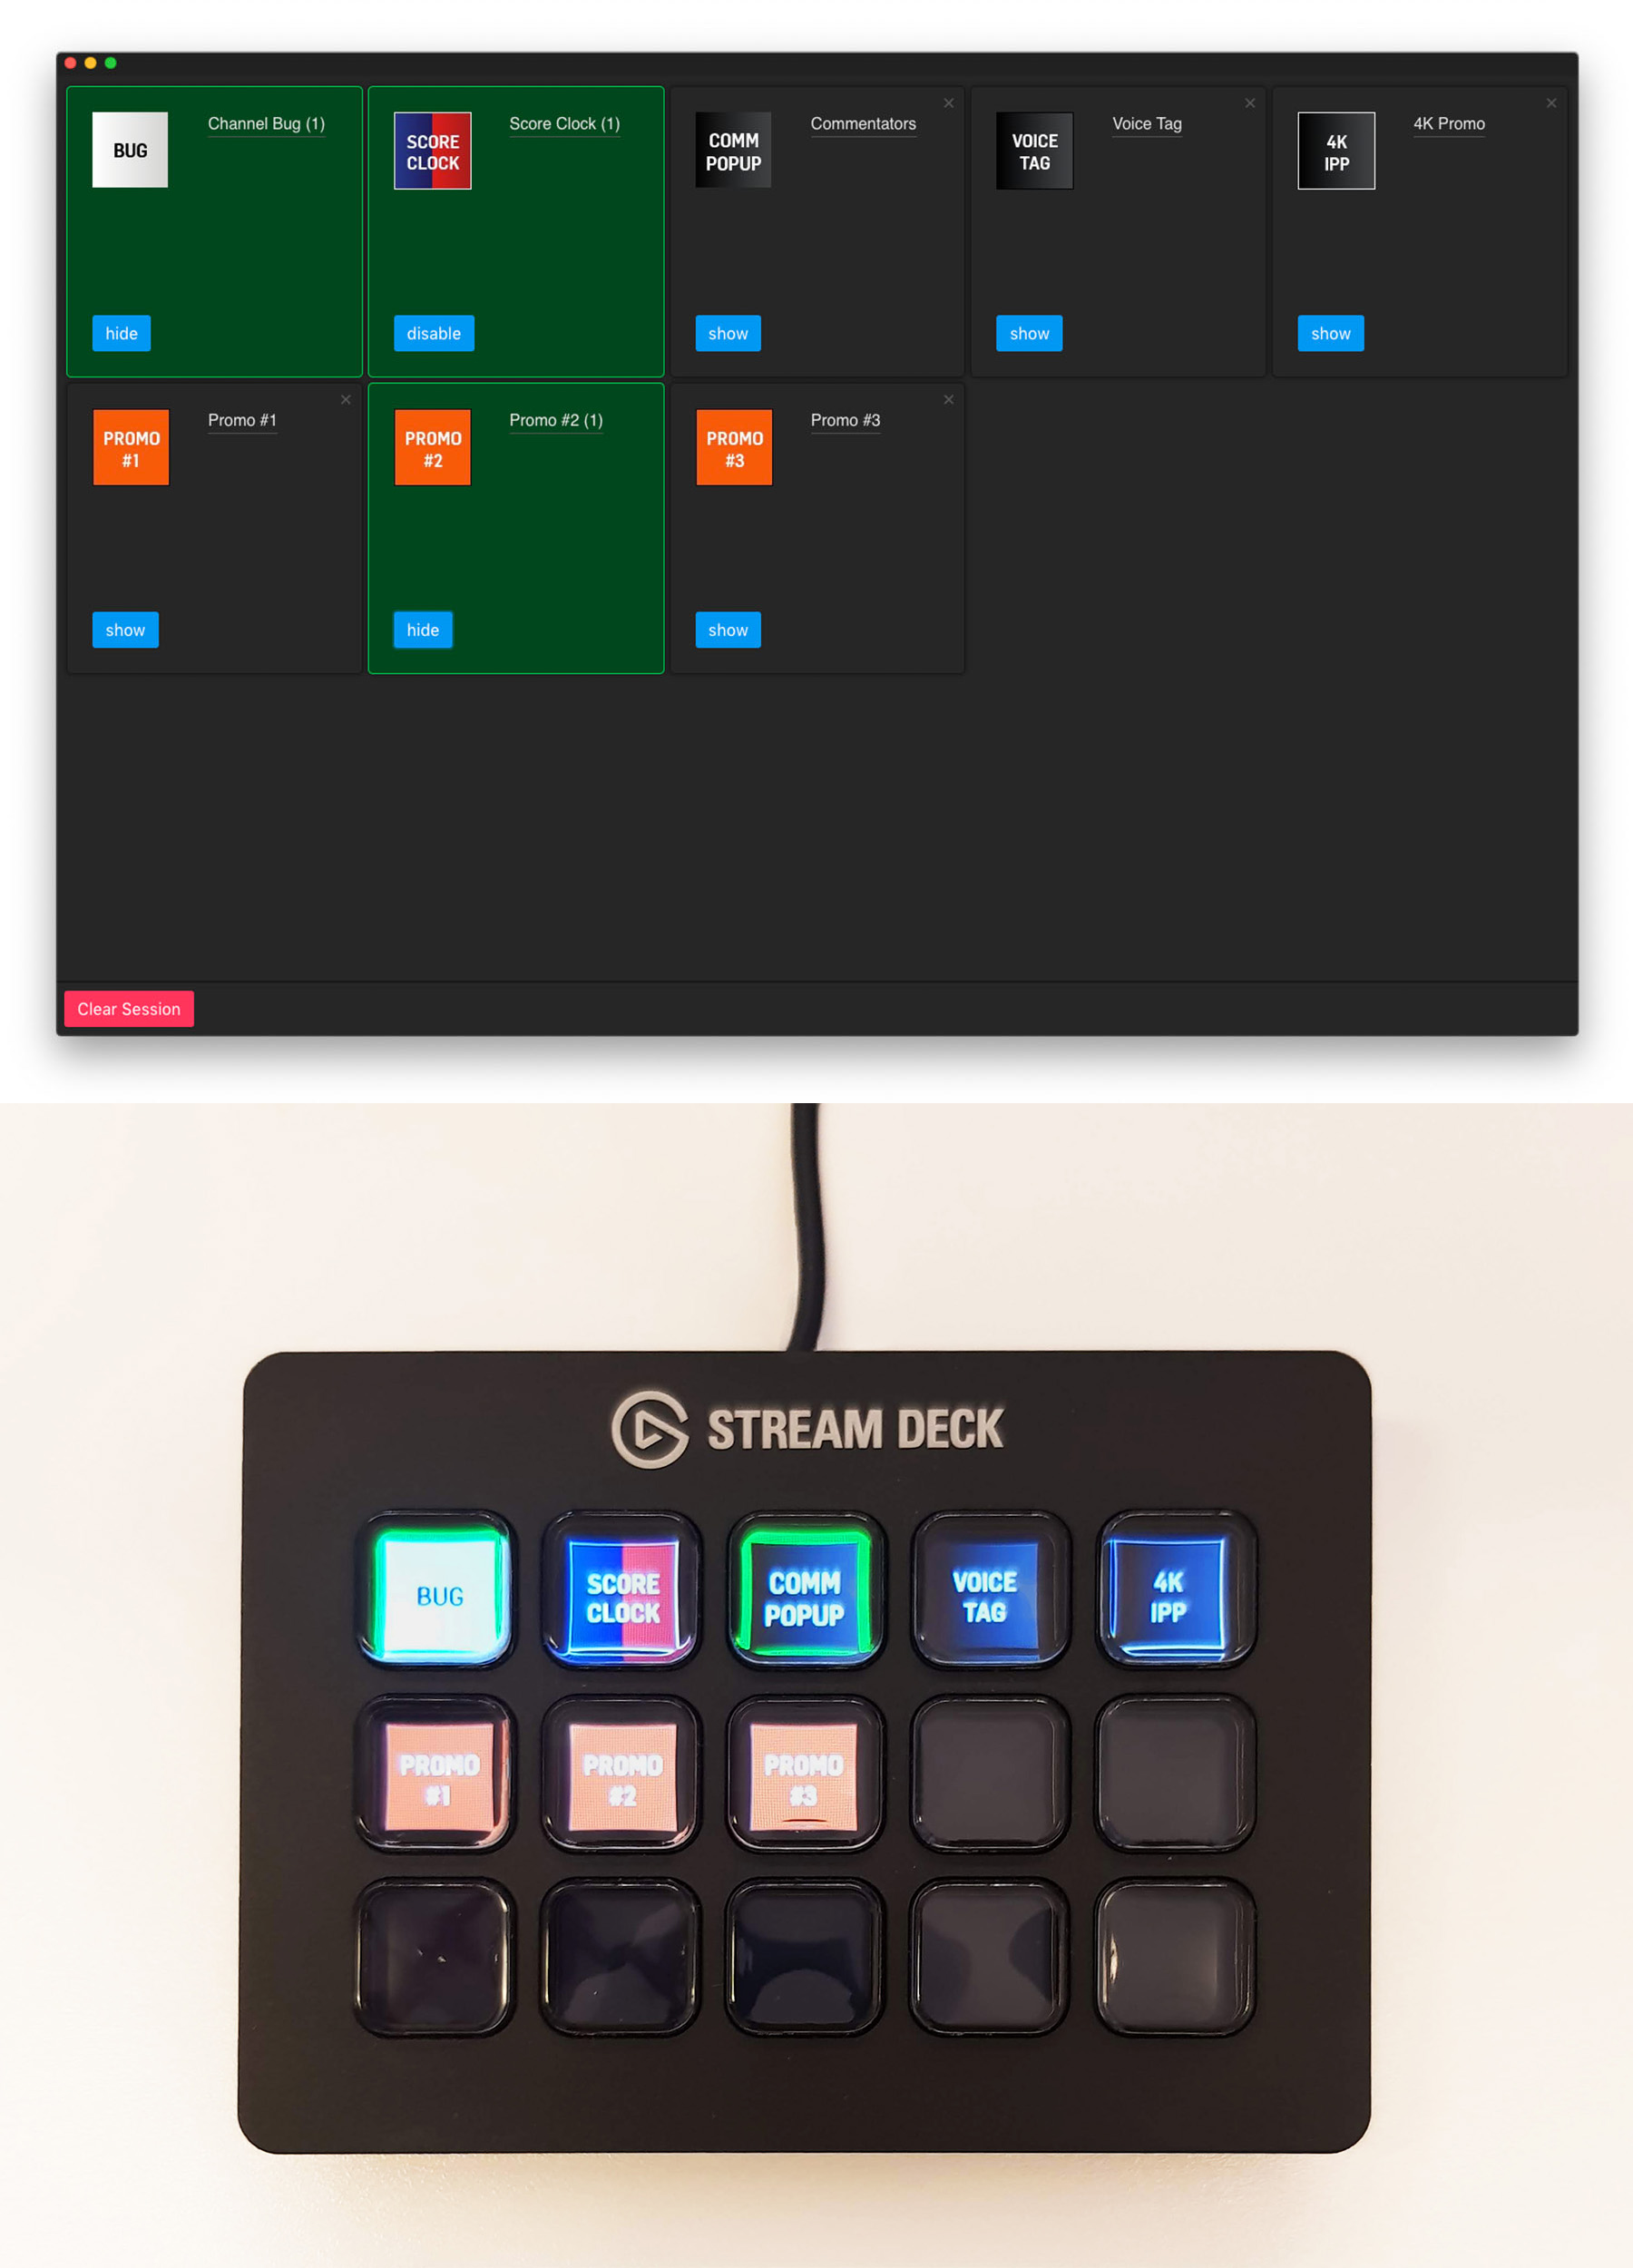
\includegraphics[width=\marginparwidth-10pt]{Figures/streamdeck.jpg}
    \caption{Trigger launcher (top) and hardware device \emph{StreamDeck} (bottom) for operating it more conveniently}
    \label{fig:streamdeck}
\end{marginfigure}

Based on the requirements, we designed a new version of our live triggering
tool, diving it into two sub-tasks, each one targeted at a different professional
(Figure~\ref{fig:triggertool}). The first tool, called \emph{Triggering Tool} allows to prepare media,
such as replay clips, or inserting on-screen labels and queueing
them for the director to launch. The second one, called \emph{Trigger Launcher}, intended for the director, can
be used for launching these events, i.e.\ inserting them into the broadcast.
For the second one, we were able to integrate support for \emph{StreamDeck}, a
hardware device intended for video-game streamers. The device is equipped with 15
buttons, where each button is backed by a $72\times72$ pixel LCD screen, plugged into the computer via USB
(Figure~\ref{fig:streamdeck}). This enabled us to map the events rendered in the
trigger launcher onto the buttons, allowing the user to conveniently launch and
modify events quickly from this console instead of having to use the mouse and
click the corresponding button on the computer screen.

\section{Object-Based Broadcasting during FA Cup Final}
After the preparation work described in the previous section, the research team
was (almost) ready to bring a unique football experience of the FA Cup Final
at Wembley Stadium to people's homes. The football experience was to be a unique, object-based broadcast, since a
multitude of media objects could be assembled in a personalized manner and rendered on
different screens at home: a single primary shared screen (main TV) coupled with
a companion device such as a tablet (Figure~\ref{fig:homeexperience}).

The deployment at Wembley Stadium was centered around our own OB vehicle, a
Mercedes Sprinter van fitted with two small work areas and basic services
such as power, cable routing, air conditioning and lighting. This vehicle was
essential as a space to safely host and operate the additional components
required for object-based broadcasting. The vehicle was provided with assistance
from BT Sport, who also provided essential access to the necessary infrastructure
and live feeds and provided a listen-only feed of the Match Director's talkback
channel within the vehicle. This enabled the team to hear and follow the
majority of vision and graphics cues given by the director throughout each
match and thus test the object-based production tools in a representative way.
The following paragraphs detail the different components deployed during the day
of the match.

\vspace{5pt}\noindent\textbf{Live Camera Feeds.} The project team requested
access to a range of live camera feeds. We had access to the clean and dirty
(Match Director's output) broadcast feeds, the main camera-wide shot, the
manager cameras, the team benches, cameras behind each goal and the Spider
cam. Each camera feed was provided in HD-SDI format through a separate coaxial cable
routed from the BT Sport production truck to the vehicle.

\begin{marginfigure}
\hspace*{-0.5cm}
    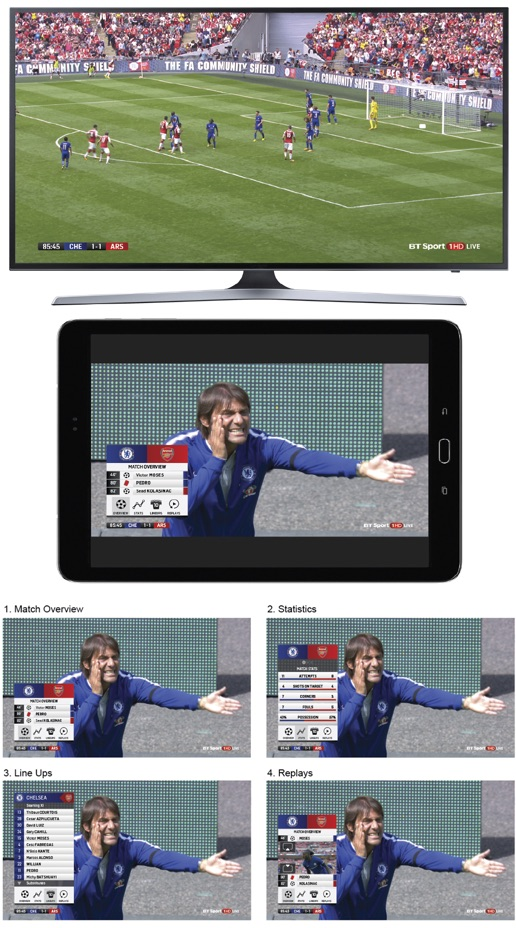
\includegraphics[width=7cm]{Figures/footballathome1.jpg}
    \caption{Experience at home as viewed by an end user: television screen (top), tablet (middle) and user-customizable screen configurations for companion screen (bottom)}
    \label{fig:homeexperience}
\end{marginfigure}

\vspace{5pt}\noindent\textbf{Live Encoding.} Two live streaming encoders were loaned for the duration
of the tests with assistance from BT Sport. Each encoder was capable of live
encoding a multi-layer DASH representation of 8 HD-SDI input streams. Once
encoded, the DASH segments were uploaded to our CDN origin server, from where
they could be consumed by the client applications. Given that the FA Cup Final
match was simultaneously broadcast free-to-air in the UK, it was agreed that
stream encryption need not be used, but instead access control was applied to
the CDN so that client apps were required to authenticate before they
could download the stream.

\vspace{5pt}\noindent\textbf{Internet Uplink.} Using additional live encoders
also necessitated providing Internet uplink capacity dedicated to the OB vehicle.
At least 100Mbps was required to upload the 3-layer MPEG-DASH representation for
8 distinct live streams, while providing headroom for audio streams and signaling.

\vspace{5pt}\noindent\textbf{Triggering Interface.} One half of the OB vehicle was dedicated to live
triggering of object-based production graphics using the production tools
described above. The tools ran on a laptop with the addition of an Elgato
Streamdeck programmable keypad. The production tools communicated with our
platform services, which were hosted off-site inside an Amazon Web Services
environment. The production tools were modified as well to enable the preview
client to display the live feed from the capture device within the primary video
player component, rather than opening the delayed MPEG-DASH stream from the CDN
origin server.

\vspace{5pt}\noindent\textbf{Tracking.} A headless camera tracking system
(ChyronHego Virtual Placement) was set up independently of the live production
tools in one half of the vehicle during the FA Cup Final event. Its purpose was
to collect the main camera pose parameters during the game. These parameters
are crucial for creating augmented graphics (graphics that blend into video as if
it was part of the three-dimensional scene). Traditionally, while burnt into
the broadcast feed, these systems are used for adding billboards, rendering
team logos on the pitch, visualizing information such as distance to goal on
free-kicks, show offside lines and more. 2-IMMERSE researchers are using the
captured data as research material to explore augmented graphics rendered in
the client. At the same venue we also captured player tracking data from the
ChyronHego TRACAB player tracking system, which can determine the location of all
players in real-time. Having synchronized data sets with video, camera
tracking and player tracking is valuable for future research in the object-based
broadcasting domain.

\vspace{5pt}\noindent\textbf{2-IMMERSE Platform.} The 2-IMMERSE
platform~\cite{jansen2018, kegel2017} was the most significant off-site
component, playing a vital role in the delivery of the end-to-end live
tests. As with all 2-IMMERSE presentations (dubbed \emph{Distributed Media
Applications}), distinct services were responsible for orchestrating the viewer experience on
end-user devices by managing layouts and and timeline sequence of on-screen objects.
Additionally, for these tests it was also necessary to orchestrate live previews for the OB truck.
Another crucial extension to the platform was the ability for timeline updates
which were created by the Live Triggering Tool to be automatically propagated to the active timelines of every client
context playing back the match, while accounting for the fact that off-site
viewers' timelines might be delayed by up to a minute due to large buffers
resulting from the MPEG-DASH live streaming configuration.

\section{Discussion}

\begin{marginfigure}
    \vspace{-8pc}
    \hspace*{-1cm}
    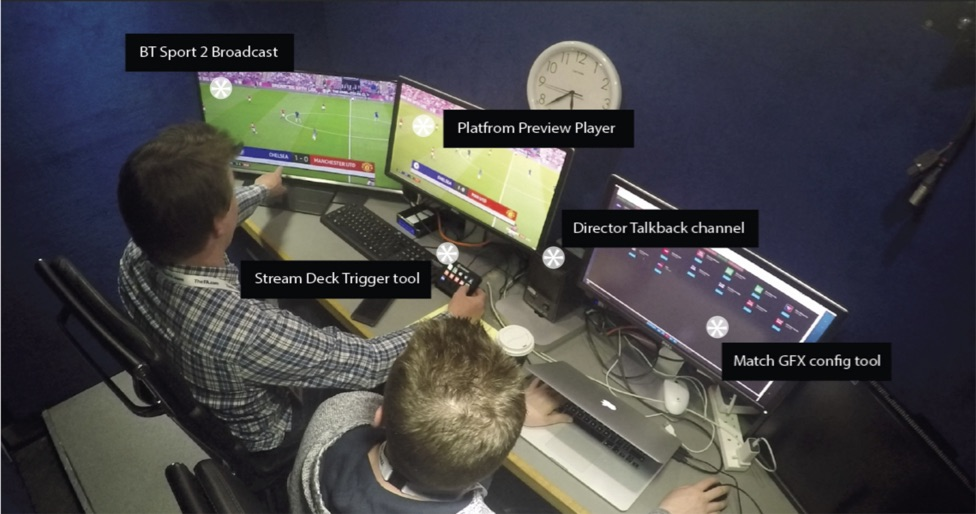
\includegraphics[width=8cm]{Figures/liveproduction.jpg}
    \caption{The setup of the system in the OB truck at the stadium}
    \label{fig:liveproduction}
\end{marginfigure}

\textbf{New challenges for the industry.} During the course of the project
(Figure~\ref{fig:timeline}), we successfully bridged the gap between lab
research and key players in the production chain (e.g. BT Sports, MoovTV),
motivating them to think about developing use cases or tools taking advantage of
OBB\@. As noted by Bentley et.al.~\cite{bentley2009}, the ethnographic-style
field study can take new concepts to real users in early stages of development,
quickly illuminating potential bottlenecks and challenges. In our trial, the
first challenge was to smooth the graphics creation workflow in this
time-critical environment. To do so, we used an existing authoring tool
(ChyronHego Prime) with a graphical interface but an XML-based storage format,
enabling a \textit{designer} to create graphics without needing a
\textit{developer}. However, the application was not specifically designed for
OBB processes. Showing that new production tools to visually create OBB assets are needed.
The second challenge addressed is the usability of the live OBB production
tool. A new version of this tool was separated into two parts. One part is
used to prepare and queue the media assets by an assistant of the director, the
other part is for the director to launch the media assets from a queue. The new
version is expected to reduce the workload for the director and result in a
smoother workflow. The third challenge we addressed was the live delivery of
the objects triggered in the OB truck to the homes of all viewers in a timely
manner.

\vspace{5pt}\noindent\textbf{Impact on the industry.} Based on the collected assets
(Figure~\ref{fig:liveproduction}) during the live event, we developed a more complete as-live multiscreen
FA Cup demonstration, showing how our tools can be used to edit broadcasts
in an OBB approach. It showed how viewers can personalize their experiences
through companion screens in home contexts. The demonstration was successfully
presented at the \emph{Future Zone} of IBC (Figure~\ref{fig:ibc}), the most
influential media exhibition in Europe. It targeted a wide audience, including
key stakeholders from broadcasting and academia, all who believed `\emph{OBB is the future}'.

\begin{marginfigure}
    \vspace{0.5pc}
    \hspace*{-1cm}
    \includegraphics[width=8cm]{Figures/IBC.jpg}
    \caption{Presenting the project at IBC 2018 in Amsterdam}
    \label{fig:ibc}
\end{marginfigure}

\section{Future Work \& Conclusion}

To help integrate the OBB approach into existing production workflows, the next
step is to develop a pre-production tool with a graphical interface, to allow
people without programming skills to author multiscreen content. The pre-production
tool aims to reduce the workload of live broadcasting by enabling producers to
create a rough storyboard of the broadcast and drop in pre-produced content ahead
of time~\cite{Li:2018_TVX}. The prototype of the pre-production tool is expected
to be tested by a group of TV professionals in December 2018. The live trial at
the 2018 FA Cup Final was a milestone to help the OBB approach to make an impact.
Through observing two live football matches, the content acquisition and distribution
was tested and the live production tools were refined to be able to trigger all graphics during the match.
Our objective of authoring a live end-to-end OBB experience and testing the
reach and scalability of our solution was achieved and can hopefully be used to
augment production workflows in future sporting events.

\begin{sidebar}
    \vspace{2pc}
    \noindent\textbf{Acknowledgements}\\
    \noindent The work presented in this paper was supported by the EU-funded
    H2020 ICT project 2-IMMERSE, under contract 687655.
\end{sidebar}

\bibliography{sample-bibliography-sigchi-a}
\bibliographystyle{ACM-Reference-Format}

\end{document}
